\section{A Unified View of Long-Term Memory Assistants}
\label{section-unified-view}


In this section, we formulate a three-stage long-term memory model for chat assistants. Despite its simplicity, this model provides a unified view of existing long-term memory assistant works. Along each of its stages, we then investigate crucial control points and propose our optimizations.


 \subsection{Long-Term Memory System: Formulation}


We formulate long-term memory as a massive key-value datastore $[(k_1, v_1), (k_2, v_2), ...]$. The keys $k_i$ can be heterogeneous, and could be discrete or continuous. In the discrete case, the key could be a sentence, a paragraph, a fact, or an entity, etc. In the continuous case, the key could be e.g., the model’s internal representation under some inputs. The values $v_i$ might repeat. As shown in \Cref{fig:main-fig-memory-unified-view}, we formulate three stages for a memory-augmented assistant: (1) \textit{indexing}, converting each history session $(t_i, S_i)$ into one or more key-value items, (2) \textit{retrieval}, formulating a retrieval query and collecting $k$ most relevant items, and (3) \textit{reading}, an LLM $\mathcal{M}$ reads the retrieval result and generates a response. {In \Cref{tab:memory-system-dimensions-comp}, we show how nine memory-augmented chat assistant systems can be viewed as instantiations of this framework. An alternative mathematical formulation is presented in \Cref{appendix-mem-system-view}. For its conciseness, the rest of this paper follows this section's formulation.}

% \vspace{-0.05in}
\subsection{Long-Term Memory System: Design Choices}
\label{section-design-choices}

We identify four crucial control points for long-term memory of chat assistants, as illustrated in \Cref{fig:main-fig-memory-unified-view}. We analyze design choices from existing works and their limitations, and propose our optimizations. Due to space constraints, we present these designs at a high level here, with detailed designs further described in \Cref{section-results} and \Cref{appendix-memory-implementation}.

\begin{figure}[t]
 \centering
 \vspace{-4mm}
 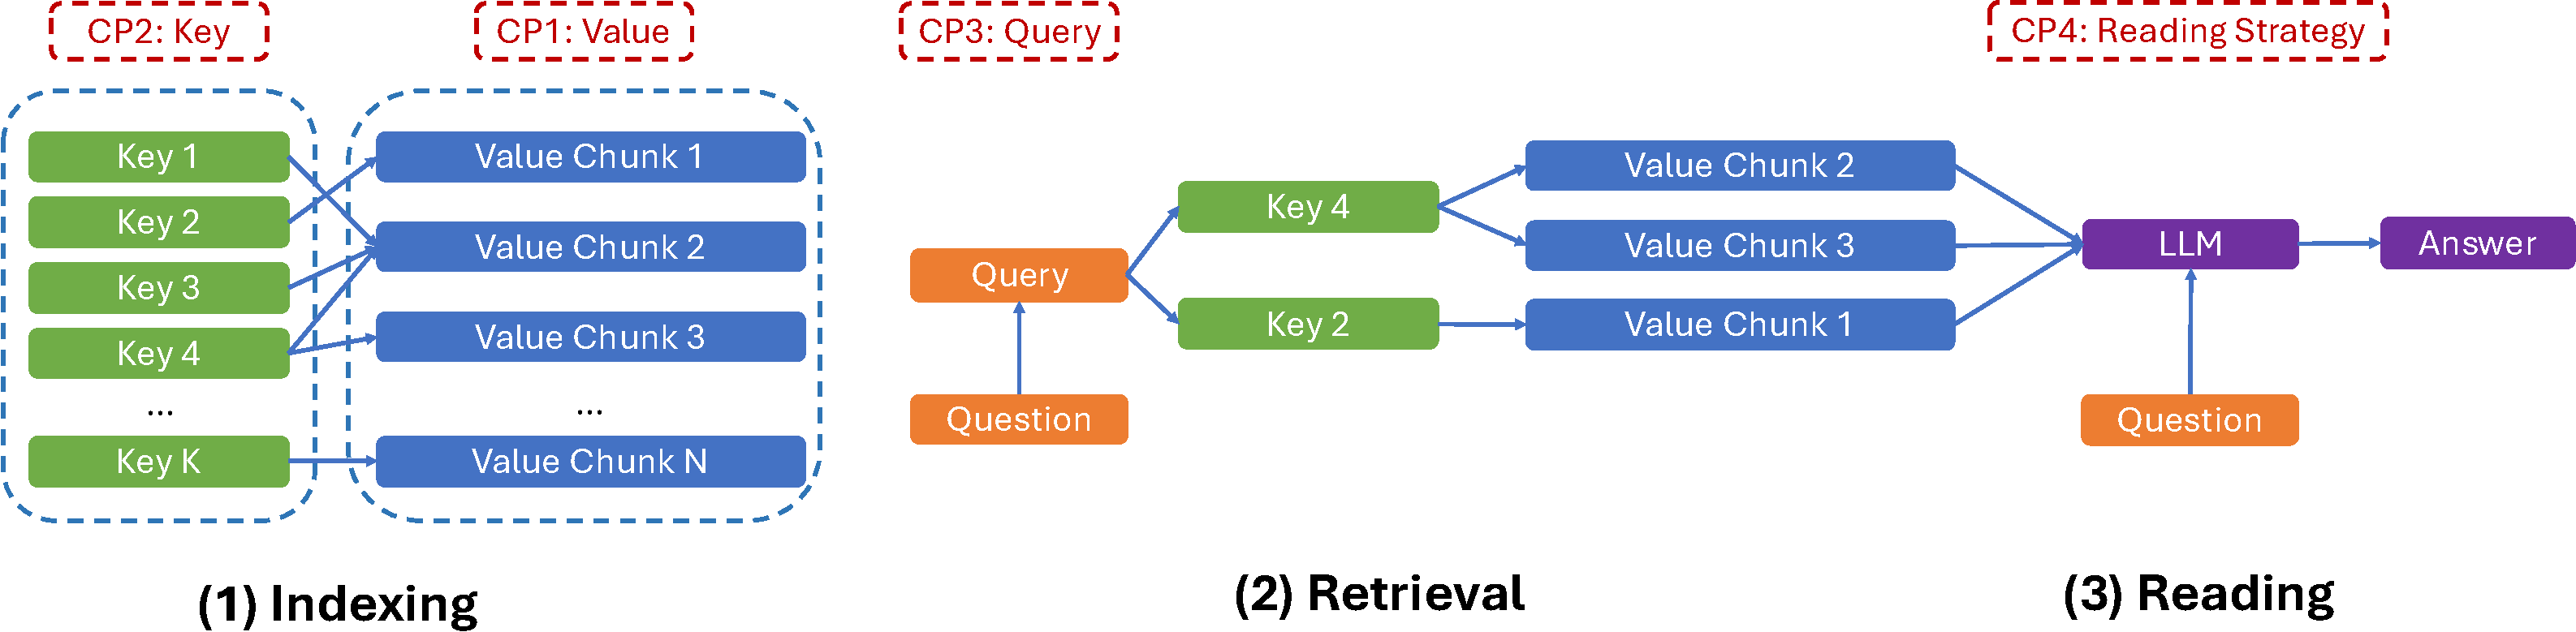
\includegraphics[width=\textwidth]{figures/mem_system_unified_view.pdf}
 % \vspace{-1mm}
 \caption{A unified view of a chat assistant with long-term memory in operation. We formulate three stages and four control points (CP). {We provide further examples in \Cref{tab:memory-system-dimensions-comp} and \Cref{appendix-mem-system-view}.}}
 \vspace{-2mm}
 \label{fig:main-fig-memory-unified-view}
 % \vspace{-1mm}
\end{figure}

\paragraph{CP 1: Value} The value represents the format and granularity of each session stored in memory. Given that user-AI chat sessions are often lengthy and cover multiple topics, storing each session as a single item can hinder effective retrieval and reading. Conversely, compressing sessions into summaries or user-specific facts, as seen in prior work such as \citet{zhong2024memorybank} and \citet{du-etal-2024-perltqa}, can lead to information loss, harming the performance of the system to answer detailed questions. In \Cref{section-value-results}, we compare three value representation strategies: storing entire sessions, decomposing sessions into individual rounds, and further applying summary/fact extraction.


\paragraph{CP 2: Key} Even when sessions are decomposed and compressed, each item still contains substantial information, with only a fraction relevant to the user's query. Therefore, using the value itself as the key, a common practice in prior works \citep{zhong2024memorybank, maharana-etal-2024-evaluating}, may be suboptimal. We introduce a key expansion approach in \Cref{section-key-results}, where summaries, keyphrases, user facts, and timestamped events are extracted from the values to augment the index. This optimization highlights the key information and enables effective retrieval with multiple pathways.


\paragraph{CP 3: Query} For straightforward user queries, the aforementioned key-value optimizations may yield high retrieval accuracy. However, when queries involve temporal references (e.g., ``Which restaurant did you recommend last weekend?"), naive similarity search proves insufficient. We address this with a time-aware indexing and query expansion strategy, where values are indexed with timestamped events, and retrieval is restricted to items within the relevant time range (\Cref{section-query-results}).


\paragraph{CP 4: Reading Strategy} Answering complex queries may require recalling numerous memory items. Although the retrieval accuracy can be enhanced through the preceding designs, it does not guarantee that the LLM can effectively reason over the extensive context \citep{DBLP:conf/icml/ShiCMSDCSZ23, DBLP:journals/tacl/LiuLHPBPL24}. In \Cref{section-reading-results}, we explore reading strategies and demonstrate that optimizations such as extracting key information before answering (Chain-of-Note, \citep{yu2023chain}) and using structured format prompting \citep{yin-etal-2023-read} are crucial for achieving high reading performance.


\setlength{\tabcolsep}{3.1pt}
\begin{table}[t]
    % \vspace{-3mm}
    \caption{{A comparison of nine memory-augmented frameworks through the lens of the proposed unified framework. We provide detailed references and discussions of each work in \Cref{appendix-mem-system-view}. For ChatGPT and Coze, we skip several designs as they are unknown.}}
    \vspace{-1mm}
    \centering
    \resizebox{\linewidth}{!}{
    \begin{tabular}{c|c|c|c|c|c|c}
        \toprule
        \textbf{Method} & \textbf{Value} & \textbf{Key} & \textbf{Query} & \textbf{Retrieval} & \textbf{Time-aware} & \textbf{Reading} \\
        \midrule
        In-context RAG \citep{shi-etal-2024-replug} & round/session & K = V & question & flat & No & direct \\
        MemoryBank \citep{zhong2024memorybank} & summary + round & K = V & question & flat & Yes & direct \\
        LD-Agent \citep{DBLP:journals/corr/abs-2406-05925} & summary + fact & K = V & keyphrase & flat & Yes & direct \\
        CoN \citep{yu2023chain} & round/session & K = V & question & flat & No & CoN \\
        ChatGPT & fact & - & - & - & No & - \\
        Coze & fact & - & - & - & No & - \\
        RAPTOR \citep{DBLP:conf/iclr/SarthiATKGM24} & round/session & node summary & question & flat/interactive & No & - \\
        MemWalker \citep{DBLP:journals/corr/abs-2310-05029} & round/session & node summary & question & interactive & No & interactive \\
        HippoRAG \citep{DBLP:journals/corr/abs-2405-14831} & round/session & entity & entity & PPR & No & direct \\
        \midrule
        Our Design & round & K = V + fact & question + time & flat & Yes & CoN \\
         \bottomrule
    \end{tabular}
    }
    \vspace{-2mm}
    \label{tab:memory-system-dimensions-comp}
\end{table}
